% This file was created by matlab2tikz.
%
%The latest updates can be retrieved from
%  http://www.mathworks.com/matlabcentral/fileexchange/22022-matlab2tikz-matlab2tikz
%where you can also make suggestions and rate matlab2tikz.
%
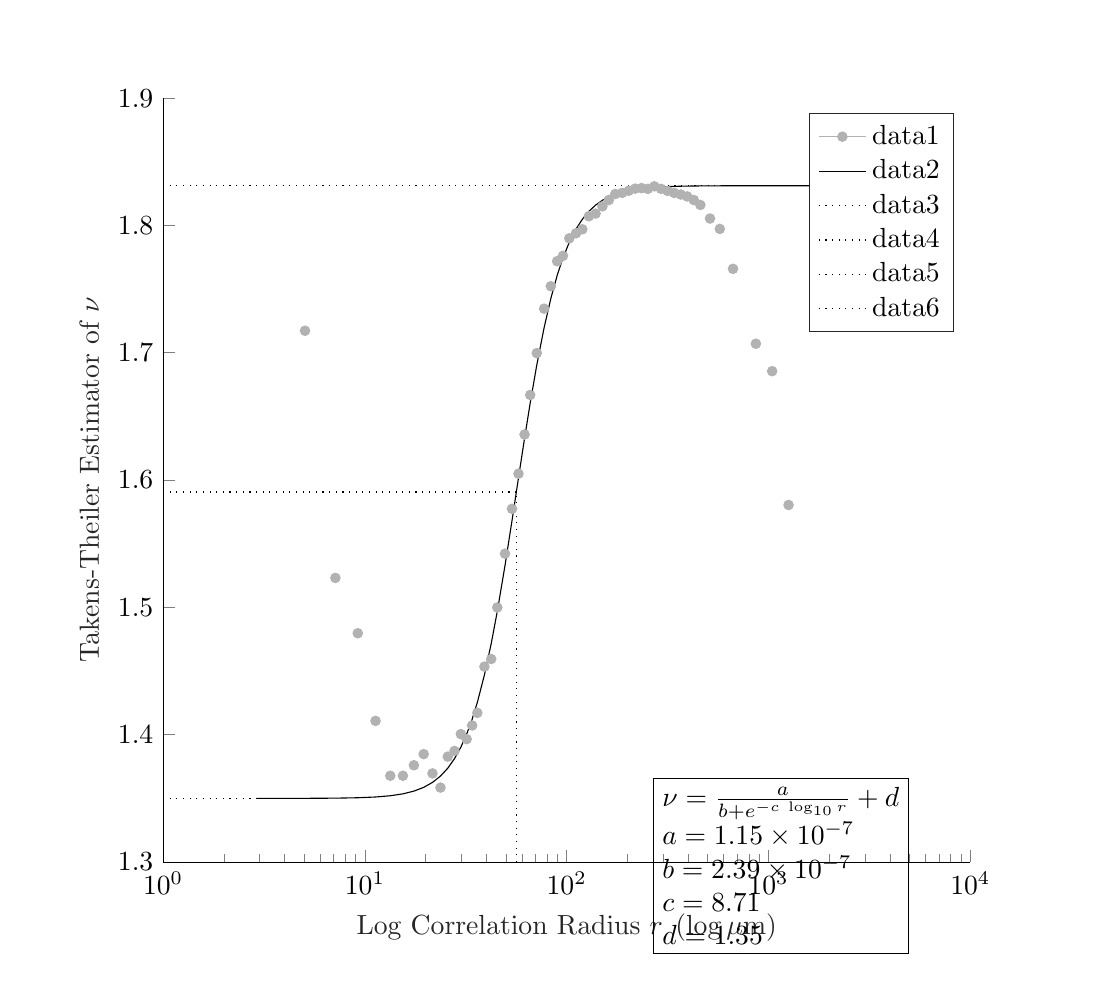
\begin{tikzpicture}

\begin{axis}[%
width=4.036in,
height=3.82in,
at={(0.677in,0.516in)},
scale only axis,
unbounded coords=jump,
xmode=log,
xmin=1,
xmax=10000,
xminorticks=true,
xlabel style={font=\color{white!15!black}},
xlabel={Log Correlation Radius \(r\;\left(\log{\mathrm{\mu}\rm{m}}\right)\)},
ymin=1.3,
ymax=1.9,
ytick={1.3,1.4,1.5,1.6,1.7,1.8,1.9},
ylabel style={font=\color{white!15!black}},
ylabel={Takens-Theiler Estimator of $\nu$},
axis background/.style={fill=white},
axis x line*=bottom,
axis y line*=left,
legend style={legend cell align=left, align=left, draw=white!15!black}
]
\addplot [color=white!70!black, draw=none, mark size=1.7pt, mark=*, mark options={solid, white!70!black}]
  table[row sep=crcr]{%
2.916108	2.12269\\
5.050848	1.717273\\
7.142978	1.523173\\
9.221544	1.479698\\
11.294039	1.410894\\
13.363287	1.367805\\
15.430595	1.367805\\
17.49665	1.376034\\
19.56185	1.38478\\
21.626438	1.369632\\
23.690576	1.358495\\
25.754372	1.382803\\
27.817901	1.387248\\
29.881219	1.400496\\
31.944367	1.396546\\
34.007375	1.407286\\
36.070268	1.417183\\
39.123699	1.453483\\
42.258425	1.459478\\
45.317112	1.499946\\
49.445023	1.542191\\
53.572331	1.577449\\
57.699167	1.605011\\
61.825624	1.635808\\
65.951773	1.666836\\
71.071729	1.699705\\
77.263115	1.734605\\
83.453703	1.75222\\
89.643657	1.771858\\
95.8331	1.776091\\
103.017487	1.789826\\
111.271603	1.793804\\
119.524875	1.796953\\
128.771859	1.807162\\
139.089504	1.809275\\
150.398837	1.814979\\
161.784893	1.819958\\
174.089471	1.824647\\
188.534919	1.825557\\
202.978739	1.827208\\
218.416322	1.828873\\
234.923254	1.829298\\
252.424512	1.828719\\
271.988665	1.83069\\
293.616057	1.828713\\
316.313757	1.827084\\
340.997698	1.825526\\
367.822887	1.824252\\
395.640793	1.822754\\
426.515118	1.819941\\
459.530012	1.816079\\
513.052783	1.805408\\
573.858712	1.797242\\
666.947836	1.765895\\
865.779756	1.707083\\
1042.636185	1.685515\\
1257.143753	1.580438\\
1825.488495	1.286141\\
2650.006157	1.001545\\
nan	nan\\
};
\addlegendentry{data1}

\addplot [color=black]
  table[row sep=crcr]{%
2.916108	1.35000659032422\\
5.050848	1.35005263443168\\
7.142978	1.35019520687396\\
9.221544	1.35051262810224\\
11.294039	1.35110235105833\\
13.363287	1.35207881226176\\
15.430595	1.35357078675198\\
17.49665	1.35571791538903\\
19.56185	1.35866617294263\\
21.626438	1.36256212888372\\
23.690576	1.36754604361816\\
25.754372	1.37374396062228\\
27.817901	1.38125925597699\\
29.881219	1.39016429149275\\
31.944367	1.40049296489154\\
34.007375	1.41223507781999\\
36.070268	1.42533337169739\\
39.123699	1.44697890059948\\
42.258425	1.47151631212949\\
45.317112	1.49704733223085\\
49.445023	1.53268125162919\\
53.572331	1.56806926176141\\
57.699167	1.60176308827037\\
61.825624	1.63276237165664\\
65.951773	1.66052393713022\\
71.071729	1.69025002443056\\
77.263115	1.7195726099709\\
83.453703	1.74260060644315\\
89.643657	1.7605187040527\\
95.8331	1.77442788095591\\
103.017487	1.78675063800696\\
111.271603	1.79719124654846\\
119.524875	1.80480716378178\\
128.771859	1.81101185086042\\
139.089504	1.81594889899595\\
150.398837	1.81975332499736\\
161.784893	1.82245780847035\\
174.089471	1.82453881353712\\
188.534919	1.82624776114739\\
202.978739	1.82743806193071\\
218.416322	1.82833682492252\\
234.923254	1.82901658849692\\
252.424512	1.82952770253217\\
271.988665	1.82993105716214\\
293.616057	1.83024219753652\\
316.313757	1.83046999692795\\
340.997698	1.83064337820421\\
367.822887	1.83077482322267\\
395.640793	1.83087038168084\\
426.515118	1.83094485860183\\
459.530012	1.83100054666111\\
513.052783	1.83105881359824\\
573.858712	1.83109774236649\\
666.947836	1.83112974987104\\
865.779756	1.83115596901588\\
1042.636185	1.83116383572225\\
1257.143753	1.83116774762459\\
1825.488495	1.83117062114567\\
2650.006157	1.83117132177317\\
nan	nan\\
};
\addlegendentry{data2}

\addplot [color=black, dotted]
  table[row sep=crcr]{%
56.2985208627579	1.3\\
56.2985208627579	1.5905889560487\\
};
\addlegendentry{data3}

\addplot [color=black, dotted]
  table[row sep=crcr]{%
1	1.5905889560487\\
56.2985208627579	1.5905889560487\\
};
\addlegendentry{data4}

\addplot [color=black, dotted]
  table[row sep=crcr]{%
1	1.83117132177317\\
2650.006157	1.83117132177317\\
};
\addlegendentry{data5}

\addplot [color=black, dotted]
  table[row sep=crcr]{%
1	1.35000659032422\\
2.916108	1.35000659032422\\
};
\addlegendentry{data6}

\end{axis}

\begin{axis}[%
width=5.208in,
height=4.688in,
at={(0in,0in)},
scale only axis,
xmin=0,
xmax=1,
ymin=0,
ymax=1,
axis line style={draw=none},
ticks=none,
axis x line*=bottom,
axis y line*=left,
legend style={legend cell align=left, align=left, draw=white!15!black}
]
\node[below right, align=left, draw=black]
at (rel axis cs:0.6,0.2) {\( \nu = \frac{a}{b+e^{-c\;\log_{10}{r}}}+d \)\\\( a = 1.15\times 10^{-7} \)\\\( b = 2.39\times 10^{-7} \)\\\( c = 8.71 \)\\\( d = 1.35 \)};
\end{axis}
\end{tikzpicture}%